\documentclass[11pt,]{article}
\usepackage{lmodern}
\usepackage{amssymb,amsmath}
\usepackage{ifxetex,ifluatex}
\usepackage{fixltx2e} % provides \textsubscript
\ifnum 0\ifxetex 1\fi\ifluatex 1\fi=0 % if pdftex
  \usepackage[T1]{fontenc}
  \usepackage[utf8]{inputenc}
\else % if luatex or xelatex
  \ifxetex
    \usepackage{mathspec}
  \else
    \usepackage{fontspec}
  \fi
  \defaultfontfeatures{Ligatures=TeX,Scale=MatchLowercase}
\fi
% use upquote if available, for straight quotes in verbatim environments
\IfFileExists{upquote.sty}{\usepackage{upquote}}{}
% use microtype if available
\IfFileExists{microtype.sty}{%
\usepackage{microtype}
\UseMicrotypeSet[protrusion]{basicmath} % disable protrusion for tt fonts
}{}
\usepackage[margin = 1.5in]{geometry}
\usepackage{hyperref}
\PassOptionsToPackage{usenames,dvipsnames}{color} % color is loaded by hyperref
\hypersetup{unicode=true,
            pdftitle={Optimization: Part 2},
            pdfauthor={Abhinav Anand, IIMB},
            colorlinks=true,
            linkcolor=blue,
            citecolor=magenta,
            urlcolor=red,
            breaklinks=true}
\urlstyle{same}  % don't use monospace font for urls
\usepackage{color}
\usepackage{fancyvrb}
\newcommand{\VerbBar}{|}
\newcommand{\VERB}{\Verb[commandchars=\\\{\}]}
\DefineVerbatimEnvironment{Highlighting}{Verbatim}{commandchars=\\\{\}}
% Add ',fontsize=\small' for more characters per line
\usepackage{framed}
\definecolor{shadecolor}{RGB}{248,248,248}
\newenvironment{Shaded}{\begin{snugshade}}{\end{snugshade}}
\newcommand{\KeywordTok}[1]{\textcolor[rgb]{0.13,0.29,0.53}{\textbf{#1}}}
\newcommand{\DataTypeTok}[1]{\textcolor[rgb]{0.13,0.29,0.53}{#1}}
\newcommand{\DecValTok}[1]{\textcolor[rgb]{0.00,0.00,0.81}{#1}}
\newcommand{\BaseNTok}[1]{\textcolor[rgb]{0.00,0.00,0.81}{#1}}
\newcommand{\FloatTok}[1]{\textcolor[rgb]{0.00,0.00,0.81}{#1}}
\newcommand{\ConstantTok}[1]{\textcolor[rgb]{0.00,0.00,0.00}{#1}}
\newcommand{\CharTok}[1]{\textcolor[rgb]{0.31,0.60,0.02}{#1}}
\newcommand{\SpecialCharTok}[1]{\textcolor[rgb]{0.00,0.00,0.00}{#1}}
\newcommand{\StringTok}[1]{\textcolor[rgb]{0.31,0.60,0.02}{#1}}
\newcommand{\VerbatimStringTok}[1]{\textcolor[rgb]{0.31,0.60,0.02}{#1}}
\newcommand{\SpecialStringTok}[1]{\textcolor[rgb]{0.31,0.60,0.02}{#1}}
\newcommand{\ImportTok}[1]{#1}
\newcommand{\CommentTok}[1]{\textcolor[rgb]{0.56,0.35,0.01}{\textit{#1}}}
\newcommand{\DocumentationTok}[1]{\textcolor[rgb]{0.56,0.35,0.01}{\textbf{\textit{#1}}}}
\newcommand{\AnnotationTok}[1]{\textcolor[rgb]{0.56,0.35,0.01}{\textbf{\textit{#1}}}}
\newcommand{\CommentVarTok}[1]{\textcolor[rgb]{0.56,0.35,0.01}{\textbf{\textit{#1}}}}
\newcommand{\OtherTok}[1]{\textcolor[rgb]{0.56,0.35,0.01}{#1}}
\newcommand{\FunctionTok}[1]{\textcolor[rgb]{0.00,0.00,0.00}{#1}}
\newcommand{\VariableTok}[1]{\textcolor[rgb]{0.00,0.00,0.00}{#1}}
\newcommand{\ControlFlowTok}[1]{\textcolor[rgb]{0.13,0.29,0.53}{\textbf{#1}}}
\newcommand{\OperatorTok}[1]{\textcolor[rgb]{0.81,0.36,0.00}{\textbf{#1}}}
\newcommand{\BuiltInTok}[1]{#1}
\newcommand{\ExtensionTok}[1]{#1}
\newcommand{\PreprocessorTok}[1]{\textcolor[rgb]{0.56,0.35,0.01}{\textit{#1}}}
\newcommand{\AttributeTok}[1]{\textcolor[rgb]{0.77,0.63,0.00}{#1}}
\newcommand{\RegionMarkerTok}[1]{#1}
\newcommand{\InformationTok}[1]{\textcolor[rgb]{0.56,0.35,0.01}{\textbf{\textit{#1}}}}
\newcommand{\WarningTok}[1]{\textcolor[rgb]{0.56,0.35,0.01}{\textbf{\textit{#1}}}}
\newcommand{\AlertTok}[1]{\textcolor[rgb]{0.94,0.16,0.16}{#1}}
\newcommand{\ErrorTok}[1]{\textcolor[rgb]{0.64,0.00,0.00}{\textbf{#1}}}
\newcommand{\NormalTok}[1]{#1}
\usepackage{graphicx,grffile}
\makeatletter
\def\maxwidth{\ifdim\Gin@nat@width>\linewidth\linewidth\else\Gin@nat@width\fi}
\def\maxheight{\ifdim\Gin@nat@height>\textheight\textheight\else\Gin@nat@height\fi}
\makeatother
% Scale images if necessary, so that they will not overflow the page
% margins by default, and it is still possible to overwrite the defaults
% using explicit options in \includegraphics[width, height, ...]{}
\setkeys{Gin}{width=\maxwidth,height=\maxheight,keepaspectratio}
\IfFileExists{parskip.sty}{%
\usepackage{parskip}
}{% else
\setlength{\parindent}{0pt}
\setlength{\parskip}{6pt plus 2pt minus 1pt}
}
\setlength{\emergencystretch}{3em}  % prevent overfull lines
\providecommand{\tightlist}{%
  \setlength{\itemsep}{0pt}\setlength{\parskip}{0pt}}
\setcounter{secnumdepth}{0}
% Redefines (sub)paragraphs to behave more like sections
\ifx\paragraph\undefined\else
\let\oldparagraph\paragraph
\renewcommand{\paragraph}[1]{\oldparagraph{#1}\mbox{}}
\fi
\ifx\subparagraph\undefined\else
\let\oldsubparagraph\subparagraph
\renewcommand{\subparagraph}[1]{\oldsubparagraph{#1}\mbox{}}
\fi

%%% Use protect on footnotes to avoid problems with footnotes in titles
\let\rmarkdownfootnote\footnote%
\def\footnote{\protect\rmarkdownfootnote}

%%% Change title format to be more compact
\usepackage{titling}

% Create subtitle command for use in maketitle
\newcommand{\subtitle}[1]{
  \posttitle{
    \begin{center}\large#1\end{center}
    }
}

\setlength{\droptitle}{-2em}
  \title{Optimization: Part 2}
  \pretitle{\vspace{\droptitle}\centering\huge}
  \posttitle{\par}
  \author{Abhinav Anand, IIMB}
  \preauthor{\centering\large\emph}
  \postauthor{\par}
  \predate{\centering\large\emph}
  \postdate{\par}
  \date{2018/06/14}

\linespread{1.25}
\usepackage{amsmath}

\begin{document}
\maketitle

\section{Background}\label{background}

The problems seeking to maximize profits or minimize costs often feature
nontrivial constraints which the optimal needs to satisfy. The solution
must lie at the intersection of constraints (for equality constraints)
or on one side of the constraint surface (for inequality constrints).

The problem in a general form is:

\[
\max f(x): x\in \mathbb{R}^n, x\geq 0
\] \[
g_1(x_1,\hdots,x_n)\leq b_1,\hdots,g_k(x_1,\hdots,x_n)\leq b_k
\] \[
h_1(x_1,\hdots,x_n)= c_1,\hdots,h_m(x_1,\hdots,x_n)= c_m
\]

The objective function \(f\) is real valued, i.e.,
\(f:\mathbb{R}^n \to \mathbb{R}\); \(g(\cdot)\) are functional forms of
the \emph{inequality} constraints while \(h(\cdot)\) are functional
forms for the \emph{equality} constraints.

\section{Equality Constraints}\label{equality-constraints}

Consider the case when \(x=(x_1, x_2)\) and there is a single equality
constraint \(h_1(x) = c_1\).

\[
\max f(x): x\in \mathbb{R}^2, x\geq 0
\] \[
h_1(x) = c_1
\]

To make the illustration more concrete, consider \(f(x) = x_1x_2\) and
\(h_1(x)=c_1:x_1+ x_2=5\).

\begin{Shaded}
\begin{Highlighting}[]
\NormalTok{x_}\DecValTok{1}\NormalTok{ <-}\StringTok{ }\KeywordTok{seq}\NormalTok{(}\FloatTok{0.1}\NormalTok{, }\DecValTok{10}\NormalTok{, }\FloatTok{0.05}\NormalTok{)}
\NormalTok{x_}\DecValTok{2}\NormalTok{ <-}\StringTok{ }\KeywordTok{seq}\NormalTok{(}\FloatTok{0.1}\NormalTok{, }\DecValTok{10}\NormalTok{, }\FloatTok{0.05}\NormalTok{)}

\NormalTok{f_x_level_}\DecValTok{2}\NormalTok{ <-}\StringTok{ }\DecValTok{2}\OperatorTok{/}\NormalTok{x_}\DecValTok{2} \CommentTok{#level sets}
\NormalTok{f_x_level_}\DecValTok{4}\NormalTok{ <-}\StringTok{ }\DecValTok{4}\OperatorTok{/}\NormalTok{x_}\DecValTok{2}
\NormalTok{f_x_level_}\DecValTok{6}\NormalTok{ <-}\StringTok{ }\DecValTok{6}\OperatorTok{/}\NormalTok{x_}\DecValTok{2}
\NormalTok{f_x_level_}\DecValTok{8}\NormalTok{ <-}\StringTok{ }\DecValTok{8}\OperatorTok{/}\NormalTok{x_}\DecValTok{2}

\NormalTok{x_}\DecValTok{3}\NormalTok{ <-}\StringTok{ }\DecValTok{5} \OperatorTok{-}\StringTok{ }\NormalTok{x_}\DecValTok{2} \CommentTok{#constraint set}

\NormalTok{data_obj_l <-}\StringTok{ }\KeywordTok{cbind}\NormalTok{(x_}\DecValTok{1}\NormalTok{, }
\NormalTok{                    f_x_level_}\DecValTok{2}\NormalTok{, }
\NormalTok{                    f_x_level_}\DecValTok{4}\NormalTok{, }
\NormalTok{                    f_x_level_}\DecValTok{6}\NormalTok{,}
\NormalTok{                    f_x_level_}\DecValTok{8}\NormalTok{,}
\NormalTok{                    x_}\DecValTok{3}
\NormalTok{                    ) }\OperatorTok\StringTok{ }
\StringTok{  }\NormalTok{dplyr}\OperatorTok{::}\KeywordTok{as_tibble}\NormalTok{() }\OperatorTok
\StringTok{  }\NormalTok{tidyr}\OperatorTok{::}\KeywordTok{gather}\NormalTok{(.,}
\NormalTok{                f_x_level_}\DecValTok{2}\OperatorTok{:}\NormalTok{x_}\DecValTok{3}\NormalTok{,}
                \DataTypeTok{key =} \StringTok{"f"}\NormalTok{,}
                \DataTypeTok{value =} \StringTok{"levels"}\NormalTok{)}

\KeywordTok{ggplot}\NormalTok{(data_obj_l, }\KeywordTok{aes}\NormalTok{(x_}\DecValTok{1}\NormalTok{, levels, }\DataTypeTok{color =}\NormalTok{ f)) }\OperatorTok{+}
\StringTok{  }\KeywordTok{geom_line}\NormalTok{() }\OperatorTok{+}
\StringTok{  }\KeywordTok{scale_y_continuous}\NormalTok{(}\DataTypeTok{limits =} \KeywordTok{c}\NormalTok{(}\DecValTok{0}\NormalTok{, }\DecValTok{10}\NormalTok{)) }\OperatorTok{+}
\StringTok{  }\KeywordTok{scale_x_continuous}\NormalTok{(}\DataTypeTok{limits =} \KeywordTok{c}\NormalTok{(}\DecValTok{0}\NormalTok{, }\DecValTok{10}\NormalTok{)) }\OperatorTok{+}
\StringTok{  }\KeywordTok{theme_minimal}\NormalTok{()}
\end{Highlighting}
\end{Shaded}

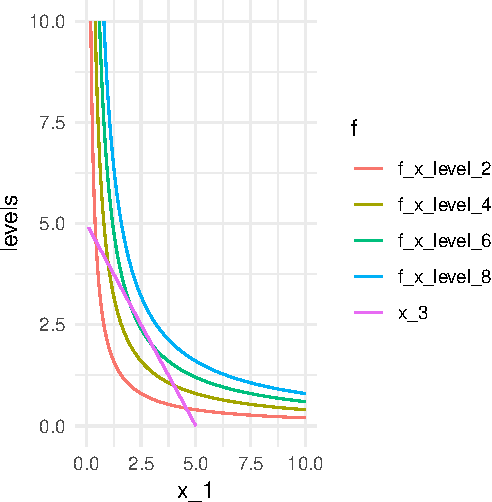
\includegraphics{Optimization_2_files/figure-latex/opt_dim_2_eq_constr-1.pdf}

Geometrically we need to find the highest valued level set for
\(f(x) = x_1x_2\) that satisfies \(x_1+x_2=5, x_1, x_2\geq 0\). The key
observation is the following: at the optimal, the levels sets and the
constraint set must be tangent---just touching (intersecting) each other
at exactly one point. (Why must this be so? What happens if the plots
cross over? Can we improve the objective function then?)

\subsection{The Lagrangian}\label{the-lagrangian}

If the curves are tangents to each other at the optimal point then it
must be so that the tangents to the curves at the optimal are in the
same direction.

The slope of the level set of \(f\) at \(x^*\) is: \[
-\frac{\frac{\partial f}{\partial x_1}(x^*)}{\frac{\partial f}{\partial x_2}(x^*)}
\] and that of the equality constraint is: \[
-\frac{\frac{\partial h}{\partial x_1}(x^*)}{\frac{\partial h}{\partial x_2}(x^*)}
\] Since they're equal \[
\frac{\frac{\partial f}{\partial x_1}(x^*)}{\frac{\partial f}{\partial x_2}(x^*)} =
\frac{\frac{\partial h}{\partial x_1}(x^*)}{\frac{\partial h}{\partial x_2}(x^*)} =
\lambda
\] This can be rearranged as: \[
\frac{\frac{\partial f}{\partial x_1}(x^*)}{\frac{\partial h}{\partial x_1}(x^*)} =
\frac{\frac{\partial f}{\partial x_2}(x^*)}{\frac{\partial h}{\partial x_2}(x^*)} =
\lambda
\] or, \[
\frac{\partial f}{\partial x_1}(x^*)-\lambda\frac{\partial h}{\partial x_1}(x^*)=0
\] \[
\frac{\partial f}{\partial x_2}(x^*)-\lambda\frac{\partial h}{\partial x_2}(x^*)=0
\] There are three unknowns:\((x_1^*, x_2^*, \lambda)\). There are two
equations above, and there is a third equation---the constraint equation
\(h(x_1, x_2) = c_1\). Together, we can find \(x^*\) and \(\lambda\).

The following function is formally referred to as the \emph{Lagrangian},
and \(\lambda\) as the Lagrange multiplier: \[
\mathcal{L}(x_1,x_2,\lambda) := f(x_1,x_2)-\lambda\cdot(h(x_1,x_2)-c)
\]

We consider the critical points of the Lagrangian:
\(\frac{\partial \mathcal{L}}{\partial x_1}(x^*), \frac{\partial \mathcal{L}}{\partial x_2}(x^*), \frac{\partial \mathcal{L}}{\partial \lambda}(x^*)=0\).

Essentially by forming the Lagrangian, we are transforming a constrained
optimization program featuring the objective function \(f(\cdot)\) into
an \emph{unconstrained} optimization program featuring the Lagrangian
\(\mathcal{L}(\cdot)\). However, there is an extra variable \(\lambda\),
the Lagrange multiplier, that is introduced in the new program.

\subsubsection{Constraint Qualification}\label{constraint-qualification}

In order for the slopes to be well-defined,
\(\frac{\partial h}{\partial x_1}(x^*)\neq 0\) and
\(\frac{\partial h}{\partial x_2}(x^*)\neq 0\). Since this is a
restriction on the constraint set, it's called a \emph{constraint
qualification}.

\textbf{Theorem:} For the function
\(f:\mathbb{R}^n\to \mathbb{R}, f\in C^1\), if \(x^*\in \mathbb{R}^n\)
is a solution of \[\max f(x): x\geq 0, h(x)=c_1\] and \(x^*\) is
\emph{not} a critical point of \(h\); then, there is a real number
\(\lambda^*\) such that \((x^*,\lambda^*)\) is a critical point of
\(\mathcal{L}=f(x)-\lambda\cdot(h(x)-c)\).

\subsection{Level-Set Gradients and
Lagrangians}\label{level-set-gradients-and-lagrangians}

\begin{Shaded}
\begin{Highlighting}[]
\NormalTok{f_x_level_star <-}\StringTok{ }\FloatTok{6.4}\OperatorTok{/}\NormalTok{x_}\DecValTok{2} \CommentTok{#set manually}

\NormalTok{data_plot_grad <-}\StringTok{ }\KeywordTok{cbind}\NormalTok{(x_}\DecValTok{1}\NormalTok{, }
\NormalTok{                        f_x_level_star,}
\NormalTok{                        x_}\DecValTok{3}
\NormalTok{                        ) }\OperatorTok
\StringTok{  }\NormalTok{dplyr}\OperatorTok{::}\KeywordTok{as_tibble}\NormalTok{() }\OperatorTok
\StringTok{  }\NormalTok{tidyr}\OperatorTok{::}\KeywordTok{gather}\NormalTok{(.,}
                \KeywordTok{c}\NormalTok{(f_x_level_star, x_}\DecValTok{3}\NormalTok{),}
                \DataTypeTok{key =} \StringTok{'f'}\NormalTok{,}
                \DataTypeTok{value =} \StringTok{'levels'}
\NormalTok{                )}

\KeywordTok{ggplot}\NormalTok{(data_plot_grad, }\KeywordTok{aes}\NormalTok{(x_}\DecValTok{1}\NormalTok{, levels, }\DataTypeTok{color =}\NormalTok{ f)) }\OperatorTok{+}
\StringTok{  }\KeywordTok{geom_line}\NormalTok{() }\OperatorTok{+}
\StringTok{  }\KeywordTok{scale_y_continuous}\NormalTok{(}\DataTypeTok{limits =} \KeywordTok{c}\NormalTok{(}\DecValTok{0}\NormalTok{, }\DecValTok{10}\NormalTok{)) }\OperatorTok{+}
\StringTok{  }\KeywordTok{geom_segment}\NormalTok{(}\KeywordTok{aes}\NormalTok{(}\DataTypeTok{x =} \FloatTok{2.5}\NormalTok{,}
                   \DataTypeTok{y =} \FloatTok{2.5}\NormalTok{,}
                   \DataTypeTok{xend =} \FloatTok{3.75}\NormalTok{, }\CommentTok{#set manually}
                   \DataTypeTok{yend =} \DecValTok{3}
\NormalTok{                   ),}
               \DataTypeTok{color =} \StringTok{"blue"}\NormalTok{,}
               \DataTypeTok{arrow =} \KeywordTok{arrow}\NormalTok{(}\DataTypeTok{length =} \KeywordTok{unit}\NormalTok{(}\FloatTok{0.015}\NormalTok{, }\StringTok{"npc"}\NormalTok{)),}
               \DataTypeTok{size =} \FloatTok{0.2}
\NormalTok{               ) }\OperatorTok{+}
\StringTok{  }\KeywordTok{theme_minimal}\NormalTok{()}
\end{Highlighting}
\end{Shaded}

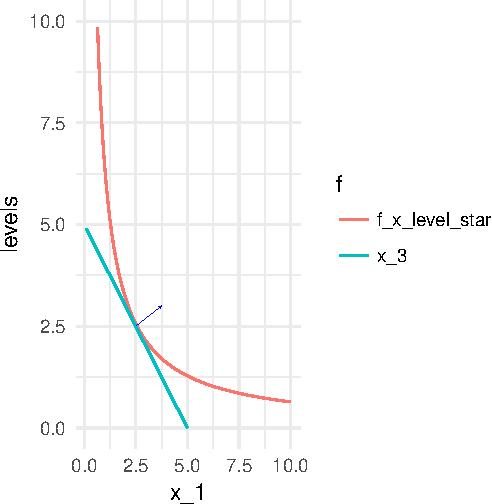
\includegraphics{Optimization_2_files/figure-latex/opt_dim_2_eq_grad-1.pdf}

The gradient of \(f\) and \(h\) are respectively
\([\frac{\partial f}{\partial x_1}, \frac{\partial f}{\partial x_2}]\)
and
\([\frac{\partial h}{\partial x_1}, \frac{\partial f}{\partial x_2}]\).
These point to the directions of maximum change and are orthogonal to
the level sets of \(f, h\).

Since the level sets and the constraints are tangent at the optimal
implies that their respective gradients---orthogonal to the
tangent---must again point in the same direction.

\[
[\frac{\partial f}{\partial x_1}, \frac{\partial f}{\partial x_2}] = 
\lambda [\frac{\partial h}{\partial x_1}, \frac{\partial h}{\partial x_1}]
\]

This yields exactly the Lagrangian function for the optimization
program.

\subsection{Several Equality
Constraints}\label{several-equality-constraints}

Consider the following variation on the maximization problem where there
are several equality constraints now:

\[
\max f(x): x\in \mathbb{R}^n, x\geq 0
\] \[
C_h = \{h_1(x)=c_1,\hdots, h_m(x)=c_m\}
\]

The generalization from one to many equality constraints is
straightforward.

\subsubsection{Constraint
Qualification}\label{constraint-qualification-1}

In the case of one constraint, the qualification is:
\[[\frac{\partial h}{\partial x_1}(x^*),\hdots,\frac{\partial h}{\partial x_n}(x^*)]\neq (0,\hdots,0)\]

Likewise, in the case of \(m\) equality constraints:
\(\{h_1(x)=c_1,\hdots, h_m(x)=c_m\}\), their \emph{Jacobian} (first
derivative matrix) must be \emph{invertible} at the critical point
\(x^*\).

\[
Dh(x^*) = \begin{bmatrix}
\frac{\partial h_1}{\partial x_1}(x^*),\hdots,\frac{\partial h_1}{\partial x_n}(x^*)\\
\frac{\partial h_2}{\partial x_1}(x^*),\hdots,\frac{\partial h_2}{\partial x_n}(x^*)\\
 \vdots \\
\frac{\partial h_m}{\partial x_1}(x^*),\hdots, \frac{\partial h_m}{\partial x_n}(x^*)
\end{bmatrix}
\]

For the constraint Jacobian at the critical point required to be
invertible implies that the matrix above must have \emph{full rank},
further equivalent to the condition that the determinant be non-zero at
the critical point. More formally, it is said that \((h_1,\hdots,h_m)\)
satisfy the \emph{non-degenrate constraint qualification} (NCDQ) at
\(x^*\) if matrix \(Dh(x^*)\) is invertible at \(x^*\) (has full rank).

\subsubsection{The Geometry of the
Lagrangian}\label{the-geometry-of-the-lagrangian}

When there are \(m\) constraints: \(h_1(x)=c_1,\hdots,h_m(x)=c_m\), the
gradient of the objective function \(\nabla f(x^*)\) at the optimal must
be a linear combination of the gradients of the constraints
\(\sum_{i=1}^m \lambda_i \nabla h_i(x^*)\).

This is so because \(\nabla h_i\) gives the directions of maximum
increase of \(h_i\). If the constraints \(h_i=c_i\) are to be satisfied,
we must move in the direction where \(h_i\) are constant (and equal to
\(c_i\)) and hence in directions \emph{orthogonal} (perpendicular) to
\(\nabla h_i\) and hence in directions \emph{orthogonal} to
\(\sum_{i=1}^m \lambda_i \nabla h_i(x^*)\). In the same way, the contour
lines for \(f\) are orthogonal to \(\nabla f\).

At the optimal, the objective function \(f\) must touch (be tangent to)
the binding constraints and hence the gradient of \(f\) must lie in the
\emph{span} of the constraints' gradients:
\(\nabla f(x^*)=\sum_{i=1}^m \lambda_i \nabla h_i(x^*)\).

\textbf{Theorem:} Given
\(f, h_1, \hdots, h_m:\mathbb{R}^n\to \mathbb{R}\in C^1\), where \(f\)
is the objective function and \(h_i=c_i\) are equality constraints which
\(x\) must satisfy; and that \(h_i\) satisfiy the NDCQ condition; then
there are \(\lambda^*=(\lambda_1^*,\hdots,\lambda_m^*)\) such that
\((x^*,\lambda^*)\) is the critical point of the Lagrangian
\(\mathcal{L}(x,\lambda)\).

Hence \[
\mathcal{L}(x,\lambda) := f(x)-\lambda_1\cdot(h_1(x)-c_1)+\hdots+\lambda_m\cdot(h_m(x)-c_m)
\] and \[
\frac{\partial\mathcal{L}}{\partial x_1}(x^*,\lambda^*)=0,\hdots,\frac{\partial \mathcal{L}}{\partial x_n}(x^*,\lambda^*)=0
\] \[
\frac{\partial\mathcal{L}}{\partial \lambda_1}(x^*,\lambda^*)=0,\hdots,\frac{\partial \mathcal{L}}{\partial \lambda_m}(x^*,\lambda^*)=0
\] In total we get \(n+m\) equations with \(n+m\) unknowns:
\((x_1,\hdots,x_n,\lambda_1,\hdots,\lambda_m)\).

\section{Inequality Constraints}\label{inequality-constraints}

Consider now a maximization program in \(\mathbb{R}^2\) with one
inequality constraint: \[
\max f(x_1, x_2), (x_1, x_2)\geq 0, g(x_1, x_2)\leq b
\]

To make the discussion more concrete, reconsider the maximization of the
objective function \(f=x_1x_2\) with an inequality constraint
\(g(x) = x_1^2+x_2^2\leq 1\).

Again we can see that for such a maximization program, the optimal must
occur at the boundary of the constraint set \(g(x)=b\). The level sets
of \(f, g\) are tangent to each other, or equivalently their gradients
are in the same direction:

\[\nabla f(x^*) = \lambda \nabla g(x^*)\]

Additionally, however we note that \(\lambda > 0\) i.e., the gradients
point in the same direction and \emph{not} in the opposite direction as
is seen below.

\begin{Shaded}
\begin{Highlighting}[]
\NormalTok{x_}\DecValTok{4}\NormalTok{ <-}\StringTok{ }\KeywordTok{sqrt}\NormalTok{(}\DecValTok{1} \OperatorTok{-}\StringTok{ }\NormalTok{x_}\DecValTok{2}\OperatorTok{^}\DecValTok{2}\NormalTok{) }\CommentTok{#inequality constraint}

\NormalTok{f_x_level_}\DecValTok{1}\NormalTok{ <-}\StringTok{ }\DecValTok{1}\OperatorTok{/}\NormalTok{x_}\DecValTok{2}
\NormalTok{f_x_level_half <-}\StringTok{ }\DecValTok{1}\OperatorTok{/}\NormalTok{(}\DecValTok{2}\OperatorTok{*}\NormalTok{x_}\DecValTok{2}\NormalTok{)}
\NormalTok{f_x_level_qtr <-}\StringTok{ }\DecValTok{1}\OperatorTok{/}\NormalTok{(}\DecValTok{4}\OperatorTok{*}\NormalTok{x_}\DecValTok{2}\NormalTok{)}
\NormalTok{f_x_level_eighth <-}\StringTok{ }\DecValTok{1}\OperatorTok{/}\NormalTok{(}\DecValTok{8}\OperatorTok{*}\NormalTok{x_}\DecValTok{2}\NormalTok{)}

\NormalTok{data_plot_ineq <-}\StringTok{ }\KeywordTok{cbind}\NormalTok{(x_}\DecValTok{1}\NormalTok{, }
\NormalTok{                        f_x_level_half,}
\NormalTok{                        f_x_level_}\DecValTok{1}\NormalTok{,}
\NormalTok{                        f_x_level_}\DecValTok{2}\NormalTok{,}
\NormalTok{                        f_x_level_eighth,}
\NormalTok{                        f_x_level_qtr,}
\NormalTok{                        x_}\DecValTok{4}
\NormalTok{                        ) }\OperatorTok
\StringTok{  }\NormalTok{dplyr}\OperatorTok{::}\KeywordTok{as_tibble}\NormalTok{() }\OperatorTok
\StringTok{  }\NormalTok{tidyr}\OperatorTok{::}\KeywordTok{gather}\NormalTok{(.,}
\NormalTok{                f_x_level_half}\OperatorTok{:}\NormalTok{x_}\DecValTok{4}\NormalTok{,}
                \DataTypeTok{key =} \StringTok{'f'}\NormalTok{,}
                \DataTypeTok{value =} \StringTok{'levels'}
\NormalTok{                )}

\KeywordTok{ggplot}\NormalTok{(data_plot_ineq, }\KeywordTok{aes}\NormalTok{(x_}\DecValTok{1}\NormalTok{, levels, }\DataTypeTok{color =}\NormalTok{ f)) }\OperatorTok{+}
\StringTok{  }\KeywordTok{geom_line}\NormalTok{() }\OperatorTok{+}
\StringTok{  }\KeywordTok{scale_y_continuous}\NormalTok{(}\DataTypeTok{limits =} \KeywordTok{c}\NormalTok{(}\DecValTok{0}\NormalTok{, }\DecValTok{2}\NormalTok{)) }\OperatorTok{+}
\StringTok{  }\KeywordTok{scale_x_continuous}\NormalTok{(}\DataTypeTok{limits =} \KeywordTok{c}\NormalTok{(}\DecValTok{0}\NormalTok{, }\DecValTok{3}\NormalTok{)) }\OperatorTok{+}
\StringTok{  }\KeywordTok{theme_minimal}\NormalTok{()}
\end{Highlighting}
\end{Shaded}

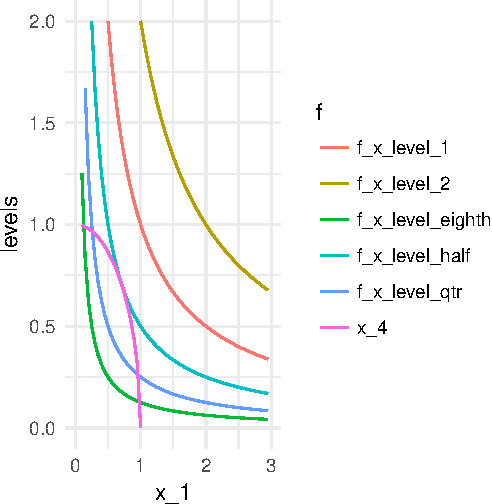
\includegraphics{Optimization_2_files/figure-latex/opt_dim_2_ineq-1.pdf}


\end{document}
